\documentclass[tikz,border=8pt]{standalone}
% Shared look for every TikZ diagram. Load with \input{../../tools/tikz-style.tex}
\usepackage[T1]{fontenc}
\usepackage{lmodern}
\renewcommand{\sfdefault}{lmr}  % diagrams use the same serif as the text
\usetikzlibrary{arrows.meta, positioning, shapes.geometric, calc, fit, backgrounds}
\definecolor{cblue}{HTML}{4C78A8}
\definecolor{corange}{HTML}{F58518}
\definecolor{cgreen}{HTML}{54A24B}
\definecolor{cred}{HTML}{E45756}
\definecolor{cpurple}{HTML}{B279A2}
\definecolor{cgrey}{HTML}{6B6B6B}
\tikzset{
  every picture/.style={font=\sffamily, line width=1.2pt},
  box/.style={draw=#1, fill=#1!12, rounded corners=4pt, align=center, inner sep=7pt, minimum height=1.1cm},
  box/.default=cgrey,
  arrow/.style={-{Stealth[length=3mm]}, draw=cgrey, line width=1.4pt},
  title/.style={font=\sffamily\bfseries\Large},
  note/.style={font=\sffamily\small, text=cgrey, align=center},
}
\AtBeginDocument{\hyphenpenalty=10000 \exhyphenpenalty=10000}

% Two ways to know the belief at time t. Top: keep the whole history and recompute from it (an archive that grows).
% Bottom: keep only the last belief and update it with the newest command and reading (a filter).
\begin{document}
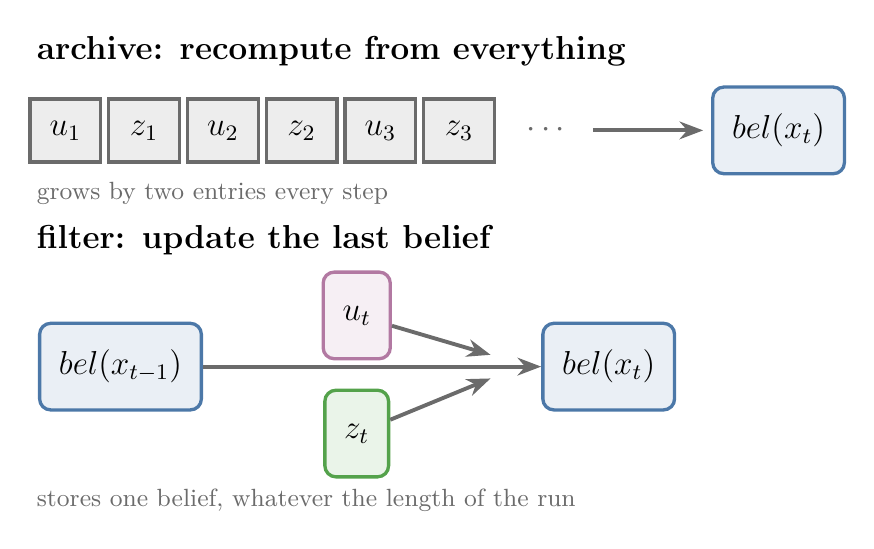
\begin{tikzpicture}[x=1cm, y=1cm, every node/.append style={font=\large}]
  \node[anchor=west, font=\large\bfseries] at (0,3.3) {archive: recompute from everything};
  \foreach \i/\l in {0/$u_1$,1/$z_1$,2/$u_2$,3/$z_2$,4/$u_3$,5/$z_3$} {
    \node[draw=cgrey, fill=cgrey!12, minimum width=0.9cm, minimum height=0.8cm] at (\i*1.0+0.5,2.3) {\l};
  }
  \node[cgrey] at (6.6,2.3) {$\cdots$};
  \draw[arrow] (7.2,2.3) -- (8.6,2.3);
  \node[box=cblue, anchor=west] at (8.7,2.3) {$\text{bel}(x_t)$};
  \node[note, anchor=west] at (0,1.5) {grows by two entries every step};
  \node[anchor=west, font=\large\bfseries] at (0,0.9) {filter: update the last belief};
  \node[box=cblue] (b1) at (1.2,-0.7) {$\text{bel}(x_{t-1})$};
  \node[box=cpurple] (u) at (4.2,-0.05) {$u_t$};
  \node[box=cgreen] (z) at (4.2,-1.55) {$z_t$};
  \node[box=cblue] (b2) at (7.4,-0.7) {$\text{bel}(x_t)$};
  \draw[arrow] (b1) -- (b2);
  \draw[arrow] (u) -- (5.9,-0.55);
  \draw[arrow] (z) -- (5.9,-0.85);
  \node[note, anchor=west] at (0,-2.4) {stores one belief, whatever the length of the run};
\end{tikzpicture}
\end{document}
